\begin{figure}
    \centering
    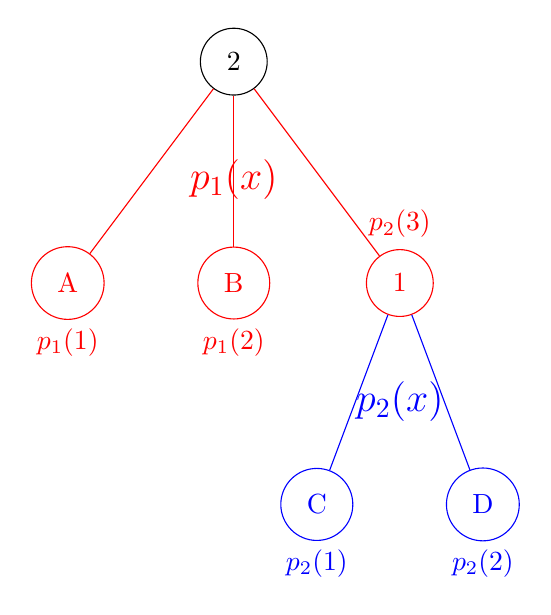
\begin{tikzpicture}
        \scoped[sibling distance=60, level distance=80, inner sep=2]{
                \tikzstyle{every node}=[circle, draw, inner sep=2mm];
                \draw (0,0) node (root) [anchor=south] {2} child [red] {node (a) {A}} child [red] {node (b) {B}} child [red] {node (subroot) {1} child [blue] {node (c) {C}} child [blue] {node (d) {D}}};
            };
            \path[red] (root) -- +(0, -1.5) node {\Large$p_1(x)$};
            \path[red] (a) -- +(0, -0.75) node {$p_1(1)$};
            \path[red] (b) -- +(0, -0.75) node {$p_1(2)$};
            \path[red] (subroot) -- +(0, 0.75) node {$p_2(3)$};

            \path[blue] (subroot) -- +(0, -1.5) node {\Large$p_2(x)$};
            \path[blue] (c) -- +(0, -0.75) node {$p_2(1)$};
            \path[blue] (d) -- +(0, -0.75) node {$p_2(2)$};
    \end{tikzpicture}
    \caption{Distribution of Secret Sharing polynomials in the Access Tree}
    \label{fig:sample-access-tree-shamir}
\end{figure}